\chapter{Erstellung \& Ausführung eines KI-Modells zur Objektdetektion} \label{sec:ai_model}
\section{Anforderungen an das KI-Modell (Jürgens)}
Ziel dieser Teilaufgabe war die Entwicklung eines KI-Modells zur automatischen Erkennung eines Holzfliegers als Zielobjekt. Eine zentrale Anforderung bestand darin, das Modell lokal auf einem Raspberry Pi 5 zu implementieren und auch dort auszuführen. Aufgrund der fehlenden dedizierten Grafikkarte des Systems war ein leichtgewichtiges, CPU-optimiertes Modell erforderlich. Der verwendete Raspberry Pi 5 verfügt über einen 64-Bit Quad-Core ARM Cortex-A76 Prozessor und 8 GB Arbeitsspeicher. \cite{raspberrypi5website} 
Aufgrund dieser Hardwarebeschränkung und persönlicher Erfahrungen wurde entschieden, dass ein YOLO Modell des Unternehmens Ultralytics verwendet wird. Dieses hat sich auf state-of-the-art KI-Modellen der YOLO-Familie im Bereich der Objekterkennung und Bildsegmentierung spezialisiert. \cite{ultralyticsFAQ} Die Modelle von Ultralytics zeichnen sich durch eine hohe Präzision und schnelle Inferenzzeiten aus. Diese Eigenschaften sind für die lokale Ausführung auf dem Raspberry Pi 5 von großer Bedeutung, da hier die Inferenz auf der CPU durchgeführt werden muss. 
Besonders interessant sind die Open-Source Implementierungen der YOLOv8 und YOLOv11 Modelle. Diese sind bereits vortrainiert und haben bestehende Gewichte und bieten somit die Möglichkeit direkt verwendet oder auf einem eigenen Datensatz weitertrainiert zu werden. Ein weiterer Vorteil der YOLO Modelle und Ultralytics liegt in der sehr guten Dokumentation und einer geringen Einstiegshürde. Mit der Ultralytics Python Bibliothek können Modelle einfach erstellt, trainiert und evaluiert werden. Dies bildet die Grundlage für die Entwicklung und Verwendung des Modells in diesem Projekt.


\section{Modellauswahl (Jürgens)}
Die YOLOv8 und YOLOv11 Modelle von Ultralytics werden in verschiedenen Größen angeboten. Mit steigender Größe des Modells steigt zwar die Genauigkeit des Modells, aber auch die Inferenzzeit und der Speicherbedarf.
Die Modelle werden in folgenden Größen angeboten:
\begin{itemize}
    \item YOLOv8/11n - Nano 
    \item YOLOv8/11s - Small
    \item YOLOv8/11m - Medium
    \item YOLOv8/11l - Large
    \item YOLOv8/11x - Extra Large
\end{itemize}
Die Modellauswahl ist durch die Hardware des Raspberry Pi 5 begrenzt. So sind insbesondere die mittleren und großen Modelle aufgrund der hohen Inferenzzeiten nicht für die Ausführung auf der CPU des Raspberry Pi 5 geeignet. Bereits das YOLOv8m Modell hat eine Inferenzzeit von 234,7 ms. \cite{ultralyticsYOLOv8Performance} Anhand dessen wurde entschieden, dass eine Beschränkung auf die kleineren Modelle YOLOv8n, YOLOv8s, YOLO11n und YOLO11s sinnvoll ist. Diese Modelle haben eine geringere Inferenzzeit und könnten somit besser für die Ausführung auf dem Raspberry Pi 5 geeignet sein. 
Die folgenden Leistungsmetriken stammen aus der offiziellen Online-Dokumentation von Ultralytics [\cite{yolov8_ultralytics,ultralyticsYOLOv8Performance,yolo11_ultralytics}]:
\begin{itemize}
    \item YOLOv8n $\approx$ 80.4 ms
    \item YOLOv8s $\approx$ 128.4 ms
    \item YOLO11n $\approx$ 56.1 ms 
    \item YOLO11s $\approx$ 90.0 ms 
\end{itemize}

Anhand dieser Werte und persönlicher Erfahrungen wurde zunächst entschieden, dass das YOLOv8n Modell im ONNX-Format verwendet wird. Dieses Modell hat mit einer Inferenzzeit von 80,4 ms eine vertretbare Geschwindigkeit.

\subsection{Das ONNX-Format (Jürgens)}
ONNX steht für Open Neural Network Exchange und stellt ein Open-Source-Format für KI-Modelle bereit. Es ermöglicht KI-Modelle über verschiedene Frameworks und Plattformen hinweg zu verwenden. Modelle können beispielweise in einem Framework mit PyTorch trainiert und anschließend in das ONNX-Format exportiert werden. Oftmals ermöglicht die Verwendung des ONNX-Formats eine bessere Performance von KI-Modellen auf verschiedenen Hardwareplattformen durch optimierte Inferenzmaschinen. \cite{ultralyticsGlossaryONNX}

Der Ansatz für dieses Projekt war es, ein Modell auf einer leistungsstarken Maschine mit dedizierter Grafikkarte zu trainieren und dieses anschließend in das ONNX-Format zu exportieren. Die Python Bibliothek von Ultralytics bietet unter Anderem die Möglichkeit ein Modell zu trainieren und anschließend in das ONNX-Format zu exportieren. Nach dem Training hat das Modell zunächst das PyTorch-Format mit der Dateiendung \texttt{.pt}.
Nach dem Export in das ONNX-Format hat das Modell die Dateiendung \texttt{.onnx}. Dieses Format kann beispielsweise mit Tools wie NVIDIA TensorRT oder Intels OpenVINO optimiert werden. Laufzeitumgebungen wie ONNX Runtime sind dabei für Hochleistungsinferenz über verschiedene Hardware optimiert. \cite{ultralyticsGlossaryONNX}


\section{Trainingsdaten \& Annotation (Jürgens)}
Die Qualität und Performance eines KI-Modells hängt maßgeblich von der Qualität der Trainingsdaten ab. Der erste Schritt ist es, einen qualitativ hochwertigen Datensatz zum Trainieren des Modells zu erstellen. Das Ziel ist es endgültig einen Holzflieger auf einem Bild zu erkennen. Die Trainingsdaten wurden direkt mit dem Raspberry Camera Module 3 aufgenommen, welches mit einer Auflösung von 11,9 Megapixeln und einer Bittiefe von 24 Bit bei einer Bildgröße von 4608x2592 Pixeln arbeitet. \cite{raspberrypi5cammodule3} Die Kamera wird neben der Erstellung der Trainingsdaten auch für die Inferenz des Modells im späteren Verlauf verwendet. 
Um eine robuste Objekterkennung unabhängig von der räumlichen Orientierung des Zielobjekts zu gewährleisten, wurde ein Datensatz von 1.201 Bildern erstellt. Diese umfassen verschiedene Umgebungsbedingungen, Beleuchtungssituationen und Perspektiven, wobei das Zielobjekt in nahezu allen möglichen Neigungen erfasst wurde.
Für das überwachte Lernverfahren sind neben den Bilddaten entsprechende Annotationen erforderlich. Der Annotationsprozess erfordert die manuelle Markierung der zu erkennenden Objekte in einem geeigneten Tool sowie deren Konvertierung in ein kompatibles Format. Dieser arbeitsintensive Prozess ist von entscheidender Bedeutung, da die Qualität der Annotationen direkt die Modellperformanz beeinflusst. Vor Beginn des Annotationsprozesses muss zunächst die Art der Annotierung definiert werden.
Für diese Arbeit gab es zwei Arten der Annotation, die in Betracht gezogen wurden:
\begin{itemize}
    \item Bounding Box: Ein Rechteck wird um das zu erkennende Objekt gezeichnet. Diese Methode ist einfach und schnell, aber weniger präzise.
    \item Polygon: Eine komplexere Form wird um das Objekt gezeichnet. Diese Methode ist genauer, aber auch zeitaufwändiger.
\end{itemize}
Die Entscheidung fiel auf die zeitaufwändigere Polygon-Annotation. Diese ermöglicht eine genauere Erkennung des Holzfliegers weil nicht nur die äußeren Kanten sondern auch die komplexere Form des Objekts berücksichtigt wird. 
Neben der speziellen Form des Holzfliegers war diese Entscheidung auch durch die relativ geringe Anzahl vorhandener Trainingsbilder begründet. 
Zur Annotation wurde das Open-Source Tool LabelStudio verwendet. Dieses bietet eine benutzerfreundliche Oberfläche und lässt sich sehr genau personalisieren. Durch die integrierte Projektverwaltung und verschiedener unterstützter Exportformate bietet das Tool eine gute Lösung für die Annotierung.
Aufgrund fehlender Implementation der Exportfunktion für größere Datensätze (Export von Bildern und korrespondierenden Annotationen) war eine Nachbereitung des Datensatzes notwendig. Nach Abschluss der Annotation wurden die Labels im YOLO-Format exportiert und eine Ordnerstruktur erstellt, die zum Training des YOLO-Modells verwendet werden kann.
\\ Folgende Ordnerstruktur wurde erstellt: \\ 

\dirtree{%
.1 train/.
.2 images/.
.2 labels/.
.1 val/.
.2 images/.
.2 labels/.
.1 test/.
.2 images/.
.2 labels/.
}

\newpage
Die Bilder und Labels im Ordner \texttt{train} werden für das Training des Modells verwendet, die Bilder und Labels im Ordner \texttt{val} für die Validierung des Modells während des Trainings und die Bilder und Labels im Ordner \texttt{test} für die abschließende Evaluation des Modells.
Die Bilder wurden in den Ordnern \texttt{images} und die Annotationen in den Ordnern \texttt{labels} gespeichert. Die Annotationen werden in Textdateien mit der Endung \texttt{.txt} gespeichert, wobei jede Textdatei die gleiche Bezeichnung wie das zugehörige Bild hat. Beispielsweise wird das Bild \texttt{image1.jpg} im Ordner \texttt{images} durch die Textdatei \texttt{image1.txt} im Ordner \texttt{labels} annotiert.


\section{Training des Modells (Jürgens)}
Ultralytics bietet mit der Python-Bibliothek \texttt{ultralytics} eine einfache Möglichkeit, ein YOLO-Modell zu trainieren, zu validieren und zu evaluieren. Vor dem Training wird eine Konfigurationsdatei benötigt, welche die Pfade des Trainingsordners, des Validierungsordners und des Testordner enthält. Neben den Pfaden beinhaltet Sie noch die Anzahl der Klassen und den dazugehörigen Namen. In diesem Fall gibt es nur den Holzflieger als Klasse, welcher zukünftig mit der Bezeichnung 'Plane' gelabelt wird. \newline

Das Training erfolgt auf einer Mittelklasse NVIDIA Grafikkarte (RTX 3070) mit 8 GB Grafikkartenspeicher und wurden der offiziellen NVIDIA Produktseite entnommen.\cite{RTX3070Specs} Während des Trainings werden die Trainingsbilder augmentiert, um die Robustheit des Modells zu erhöhen. So werden verschiedene Transformationen auf die Bilder angewendet, wie z.B. Rotation, Skalierung oder Änderung der Helligkeit. Hiermit wird die Varianz der Trainingsbilder künstlich erhöht, was zu einer besseren Performance des Modells führt. \cite{YoloDataAugmentation} Durch das Verwenden von vortrainierten Gewichten wird die Trainingszeit verkürzt und die Performance des Modells verbessert. Diese vortrainierten Gewichte werden vor dem Trainings als \texttt{.pt} Datei heruntergeladen und bereitgestellt und bieten den Ausgangspunkt für das Training. Durch Transferlearning, also dem weitertrainieren eines vortrainierten Modells auf einen neuen Datensatz, kann die Performance des Modells weiter verbessert werden. Zudem wird die benötigte Trainingszeit reduziert. \cite{TransferLearningGlossary}


Nach Abschluss des Trainings werden automatisch die besten Gewichte des Modells unter \texttt{runs/detect/train/weights/best.pt} gespeichert. Neben den reinen Gewichten erstellt das Trainingsskript unter Anderem die Datei \texttt{results.png} in welcher verschiedene Metriken des Trainings, wie zum Beispiel die \texttt{mAP50} und \texttt{mAP50-95}, visualisiert werden. Die Metrik \texttt{mean Average Precision} wie zum Beispiel \texttt{mAP50} und \texttt{mAP50-95} geben die Genauigkeit des Modells an, wobei \texttt{mAP50} die Genauigkeit bei einer IoU-Grenze von 0,5 und \texttt{mAP50-95} bei IoU-Werten zwischen 0,5 und 0,95 angibt \cite{MAPGlossary}. IoU steht für Intersection over Union und gibt die prozentuale Schnittmenge zwischen der vorhergesagten Bounding Box und der tatsächlichen Bounding Box an.\cite{IOUGlossary}
So kann man sagen, dass ein hoher \texttt{mAP50}-Wert und \texttt{mAP50-95}-Wert gute Indikatoren sind wie gut das Modell die Objekte erkennt. \newpage



\begin{figure}[h]
  \centering
  \begin{subfigure}[b]{0.45\textwidth}
    \centering
    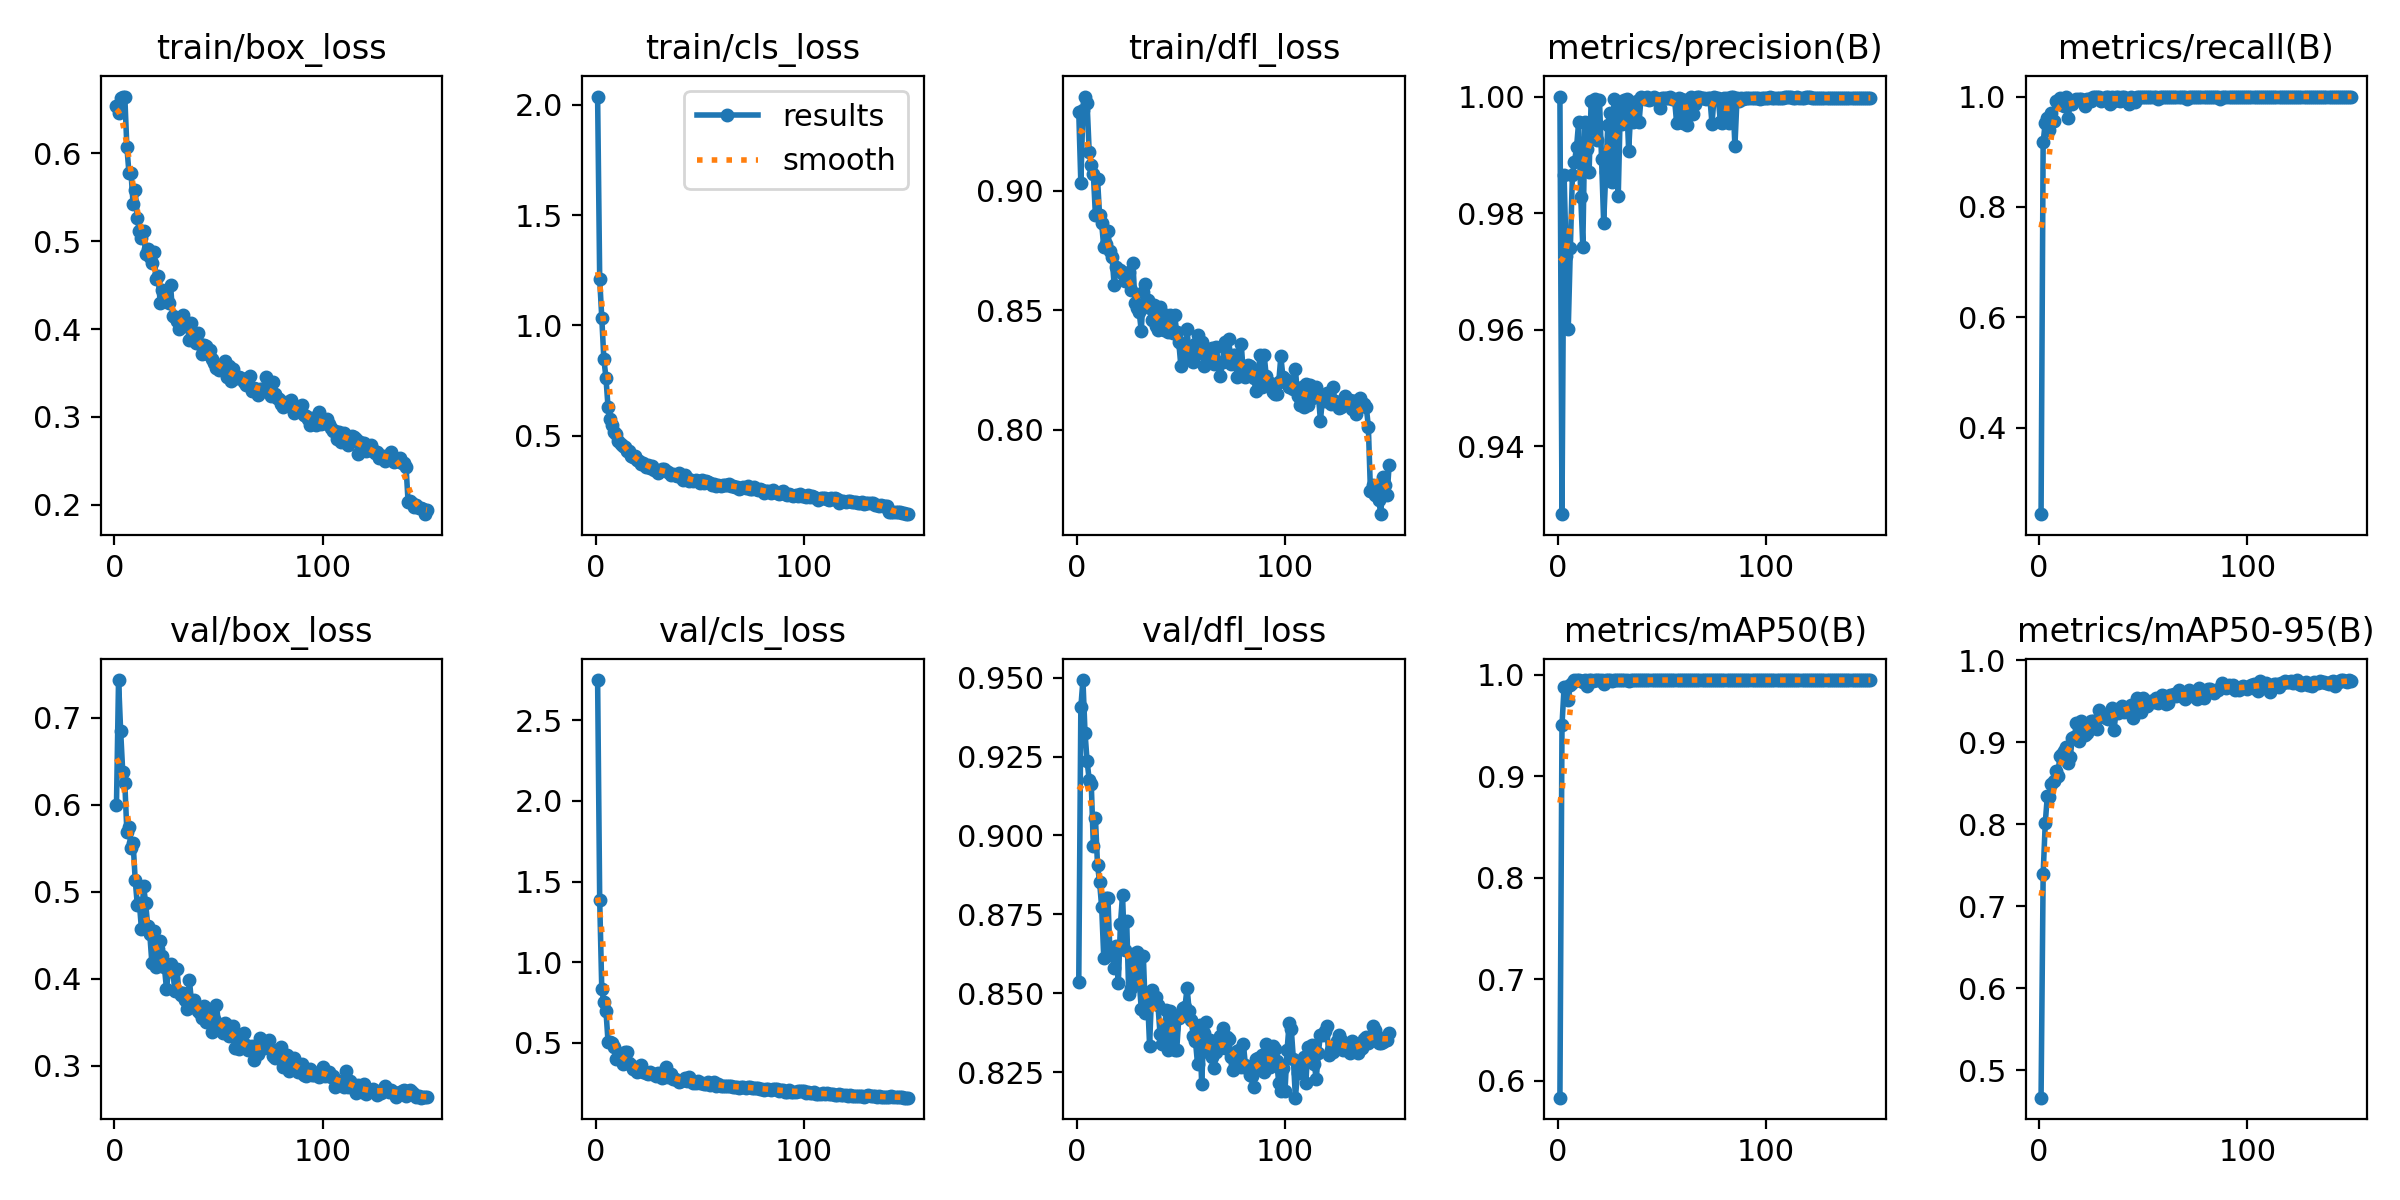
\includegraphics[width=0.9\textwidth]{images/Trainingsresults_yolov8n.png}
    \caption{YOLOv8n}
    \label{fig:Trainingsresultate yolov8n}
  \end{subfigure}
  \hfill
  \begin{subfigure}[b]{0.45\textwidth}
    \centering
    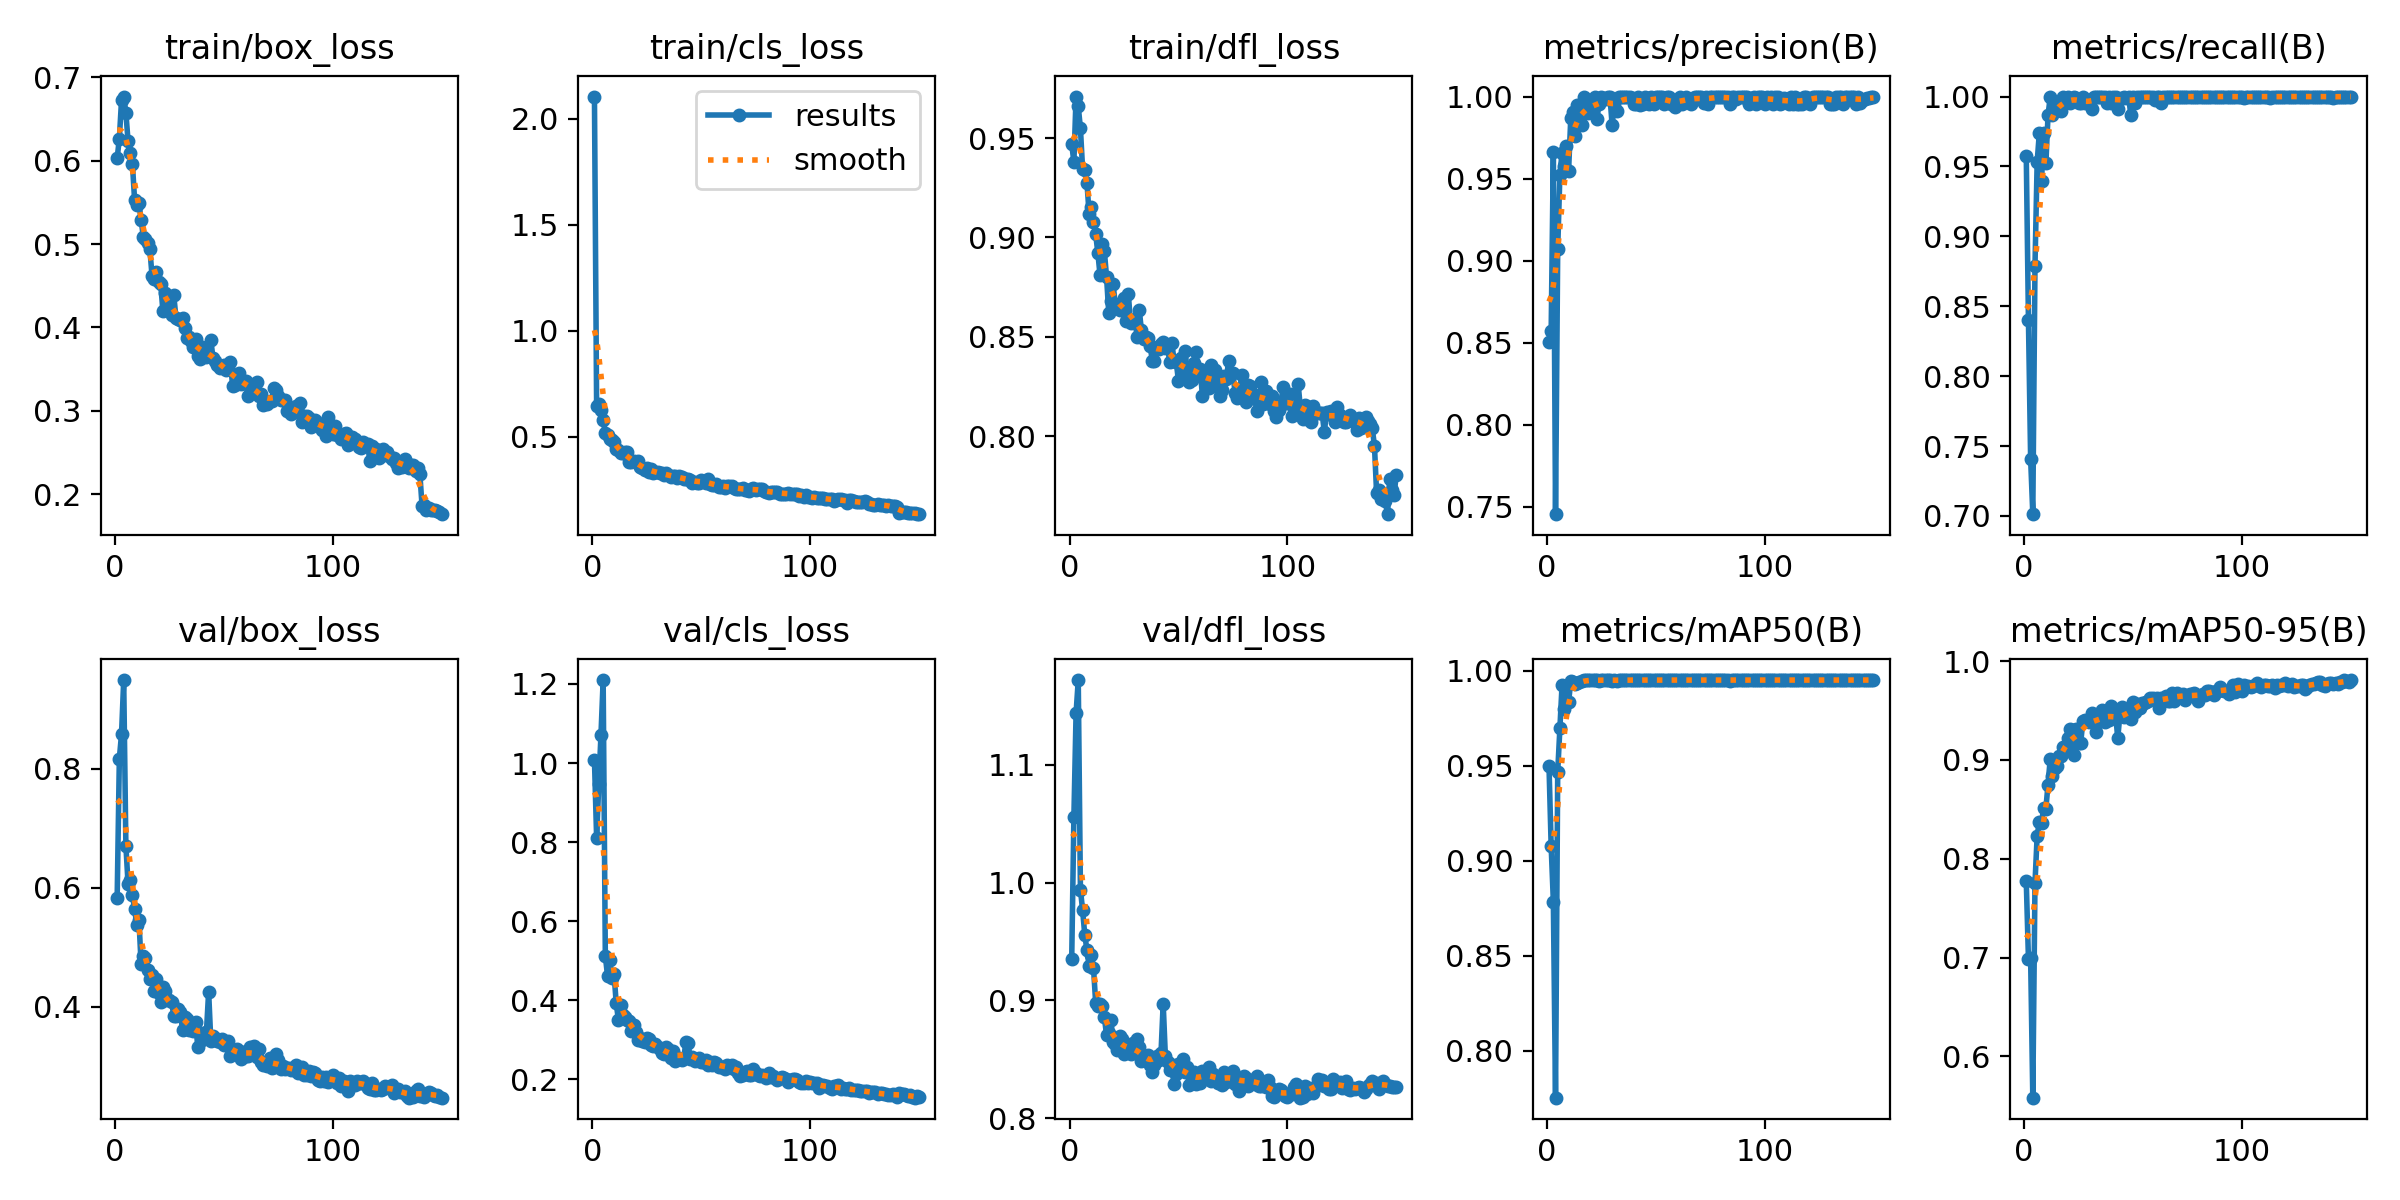
\includegraphics[width=0.9\textwidth]{images/Trainingsresults_yolov8s.png}
    \caption{YOLOv8s}
    \label{fig:Trainingsresultate yolov8s}
  \end{subfigure}
  \vskip\baselineskip
  \begin{subfigure}[b]{0.45\textwidth}
    \centering
    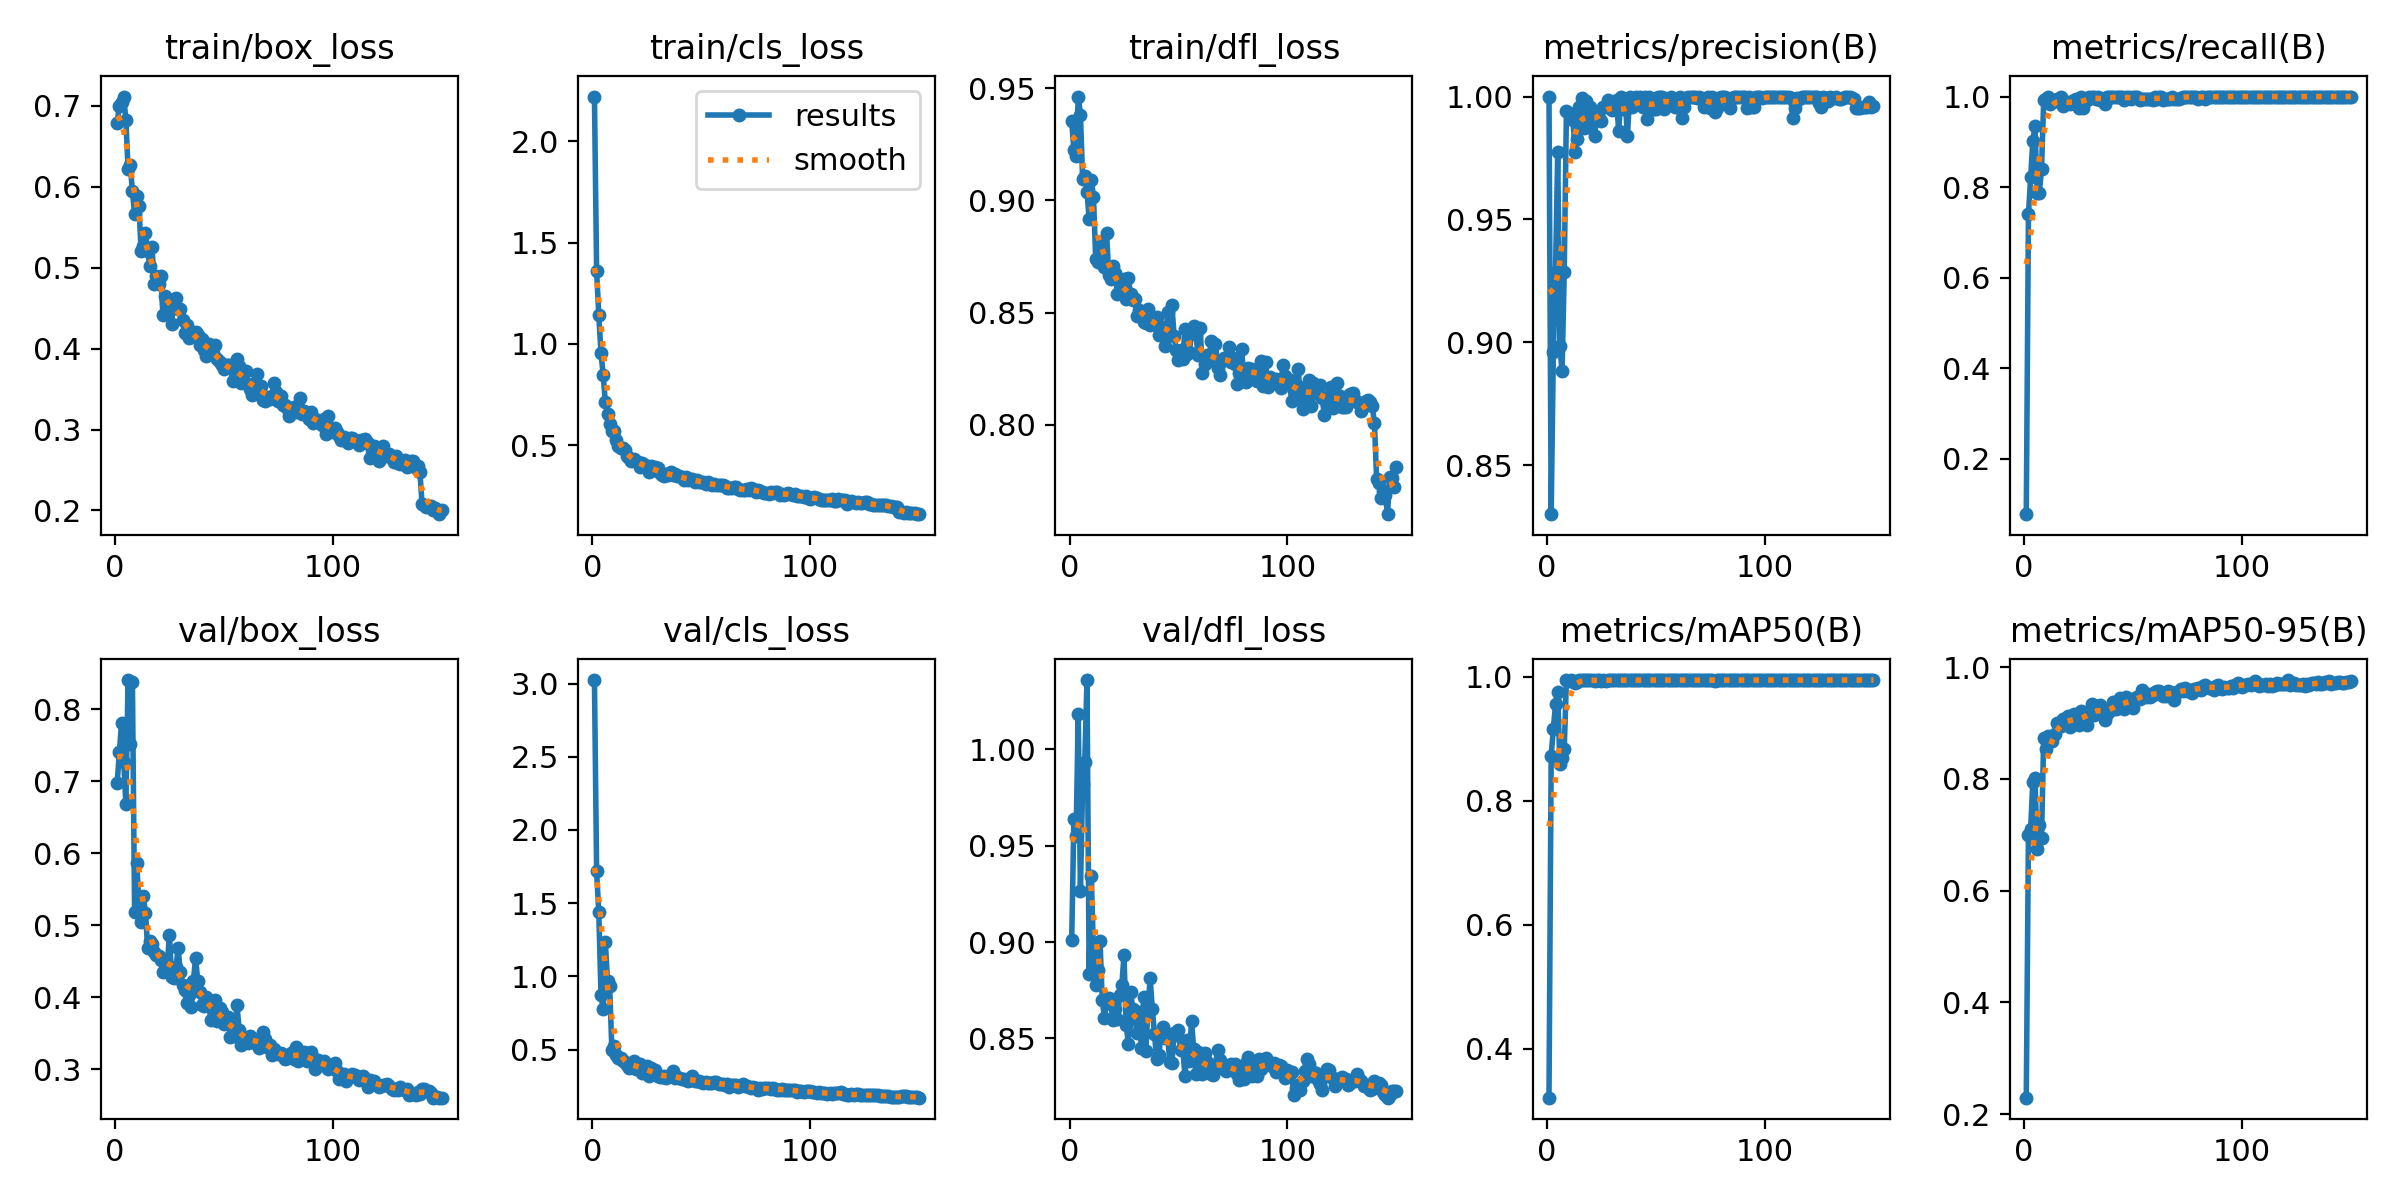
\includegraphics[width=0.9\textwidth]{images/Trainingsresults_yolo11n.png}
    \caption{YOLO11n}
    \label{fig:Trainingsresultate yolo11n}
  \end{subfigure}
  \hfill
  \begin{subfigure}[b]{0.45\textwidth}
    \centering
    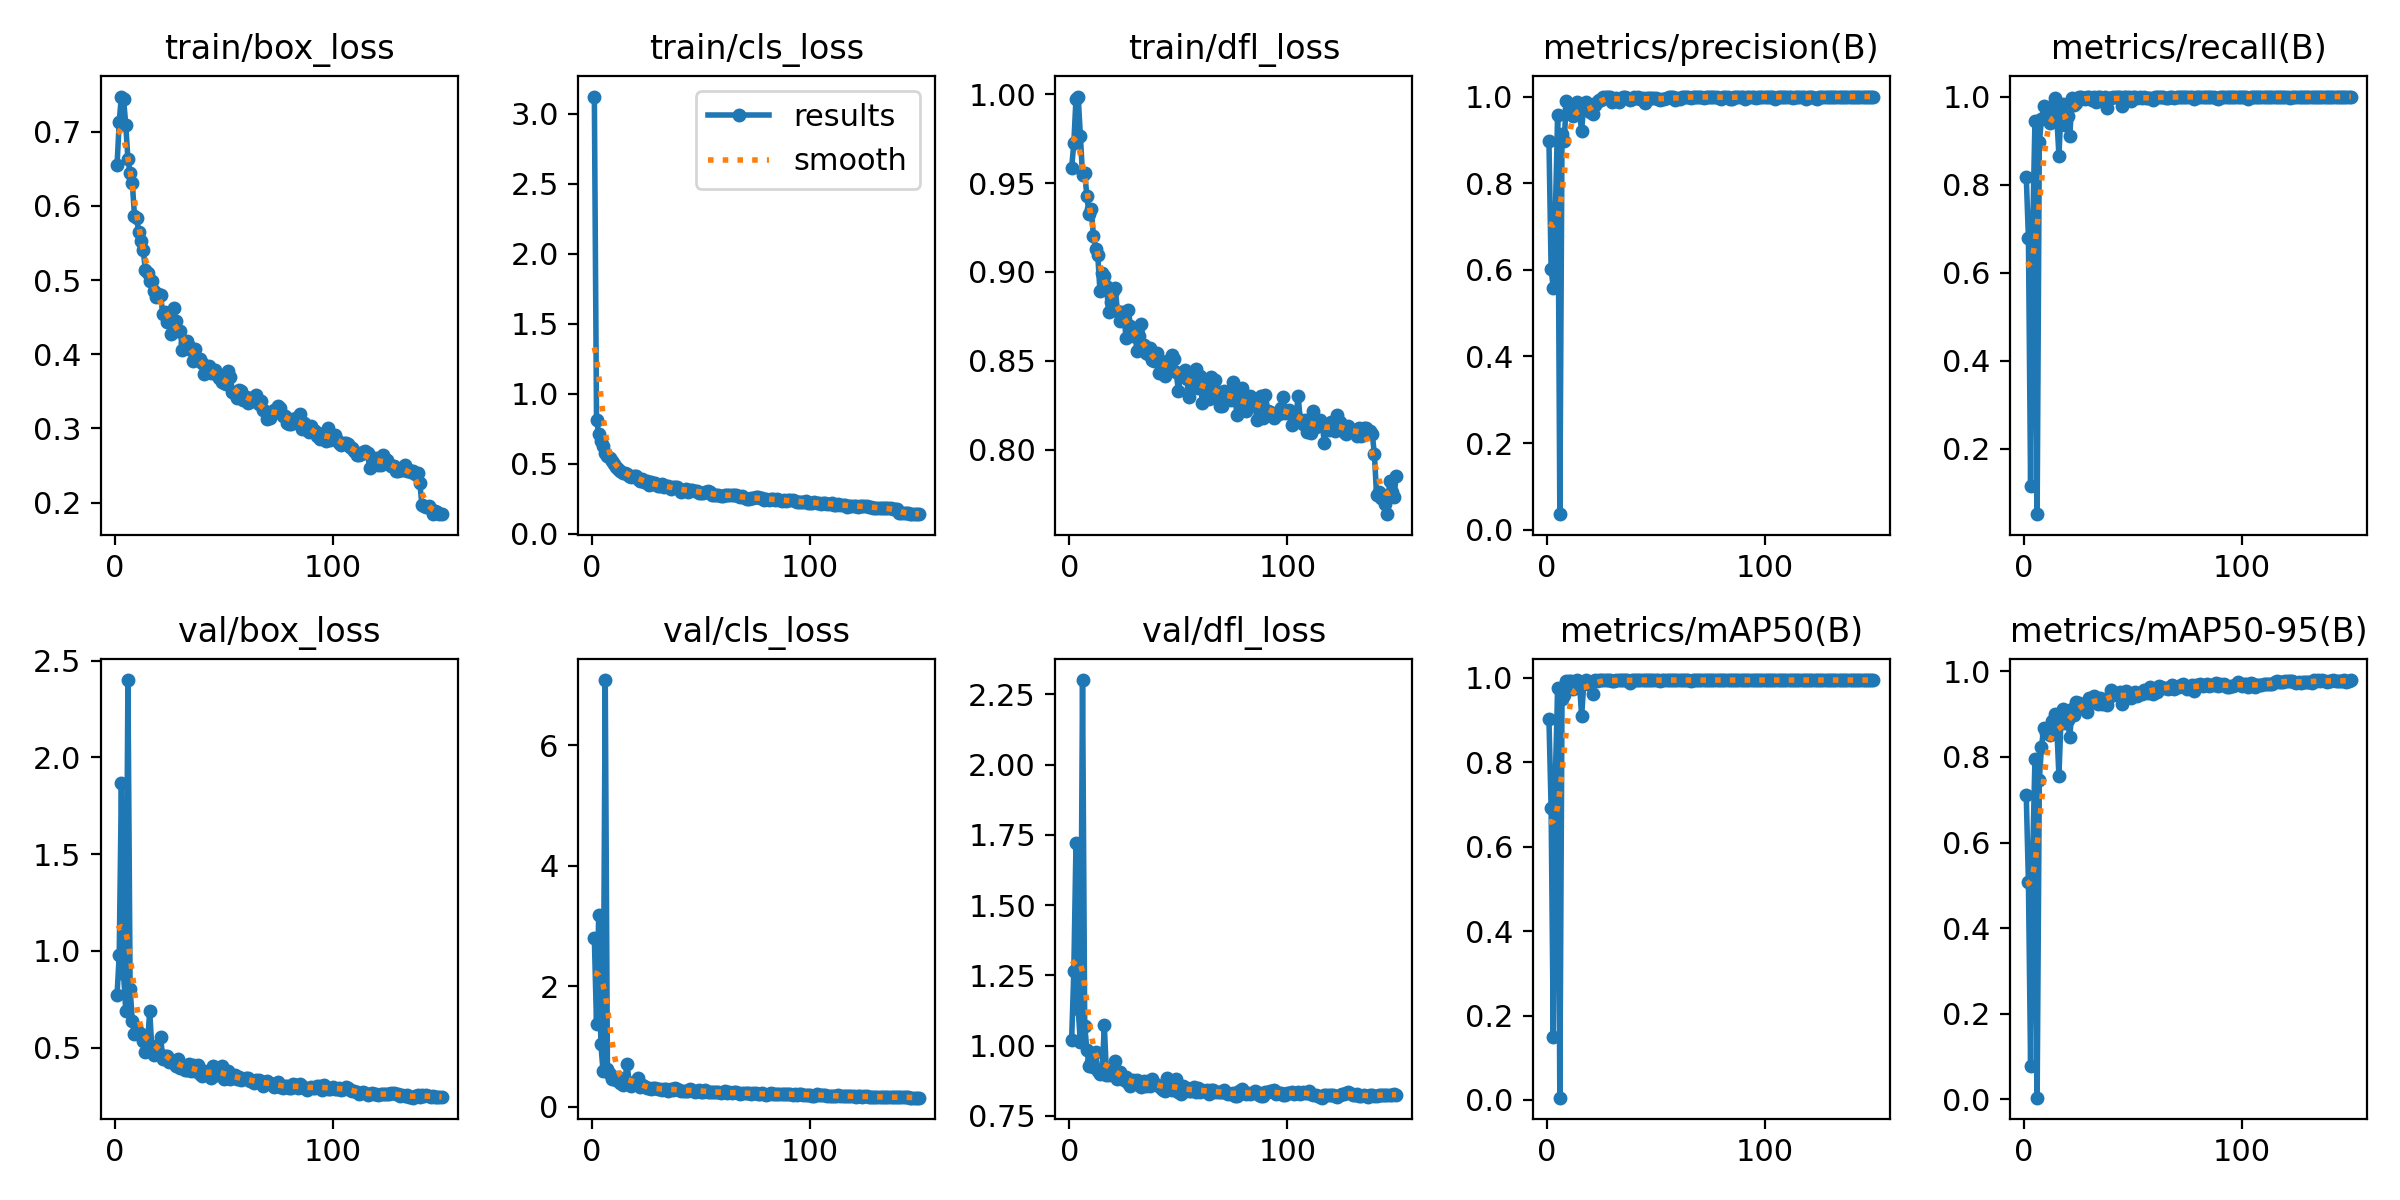
\includegraphics[width=0.9\textwidth]{images/Trainingsresults_yolo11s.png}
    \caption{YOLO11s}
    \label{fig:Trainingsresultate yolo11s}
  \end{subfigure}
  \caption{Vergleich Trainingsresultate YOLOv8n, YOLOv8s, YOLO11n und YOLO11s}
  \label{tab:Vergleich Trainingsresultate}
\end{figure}



Wie in \ref{tab:Vergleich Trainingsresultate} zu sehen ist, schneiden alle Modelle nach der Trainingsphase von 150 Epochen ähnlich gut ab. Eine Epoche stellt dabei ein vollständiger Durchlauf durch den gesamten Trainingsdatensatz dar.\cite{EpochGlossary} Anhand dieser Resultate wurde zunächst das YOLOv8n Modell ausgewählt, da es entsprechend der Trainingsmetriken trotz der geringeren Größe im Vergleich zu den s-Modellen eine ähnlich gute Performance aufweist dabei aber eine geringe Inferenzzeit aufweist. Dazu kommen positive persönliche Erfahrungen mit dem YOLOv8n Modell. 


Um das Modell schließlich auch als ONNX-Modell zu betreiben muss dieses zunächst in das ONNX-Format exportiert werden. Der Export erfolgt mit der Ultralytics Python-Bibliothek.

\section{Ausführung des Modells im ONNX-Format (Jürgens)}
Um generell ein KI-Modell im ONNX-Format auszuführen, sind einige Voraussetzung an das System zu erfüllen. Es werden verschieden Programme und Bibliotheken benötigt, um das Modell auszuführen. Um schnelle Ergebnisse und erstes Feedback zu erhalten wie die Inferenz des Modells im ONNX-Format abläuft wurde zunächst eine Laufzeitumgebung auf dem persönlichen Computer eingerichtet. Folgende Bibliotheken und Programme waren auf jeden Fall notwendig, um das Modell auszuführen:

\begin{itemize}
    \item ONNX Runtime v1.21.0
    \item OpenCV (mit GStreamer Unterstützung)
    \item CUDA 12.6 (optional, für GPU-Beschleunigung)
    \item cuDNN 9.9 (NVIDIA Deep Neural Network library, NVIDIA Developer Account erforderlich)
\end{itemize}

\newpage
Zwischen diesen Komponenten gibt es Abhängigkeiten speziell in der Versionierung. So muss beispielsweise die CUDA-Version zur eingesetzten Grafikkarte und die cuDNN-Version zur CUDA-Version passen. \\ Um den Anforderungen einer minimalen Laufzeit pro Inferenz gerecht zu werden, war die Zielprogrammiersprache C++ und nicht Python. Aufgrund fehlender Erfahrungen mit KI-Modellen im ONNX-Format wurde die Erstellung eines ersten Prototypen mit Hilfe von ChatGPT und der ONNX-Dokumentation gelöst. Es stellte sich heraus, dass die Ergebnisse der Inferenz im ONNX-Format mangelhaft sind, wobei man eine fehlerhafte Implementierung im C/C++ Code nicht ausschließen kann. Im Vergleich zu den Ergebnissen der Inferenz mit der von Ultralytics bereitgestellten Python-Bibliothek kann man die Ergebnisse der Inferenz des C/C++ Prototypen nicht verwenden. Um ein vergleichbares Ergbnis zu produzieren, werden beide Inferenzen mit dem selben Video getestet. Das Video wurde direkt mit dem Raspberry Pi 5 und dem Camera Module 3 aufgenommen.

\begin{figure}[h]
  \centering
  \begin{subfigure}[b]{0.48\textwidth}
    \centering
    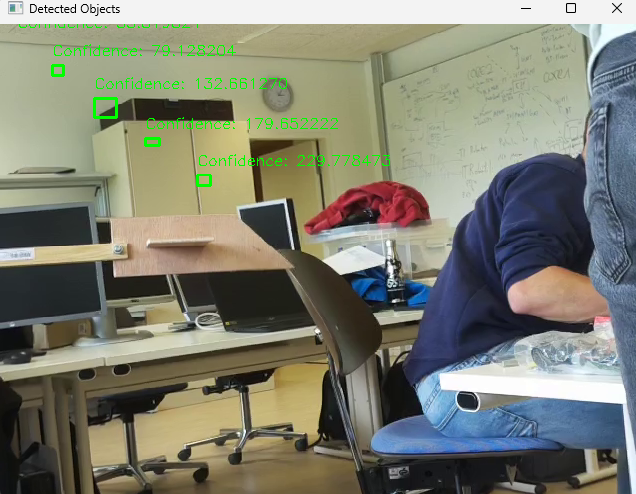
\includegraphics[width=0.9\textwidth,height=5.9cm,keepaspectratio]{images/ONNX_Inferenz.png}
    \caption{Inferenz im ONNX-Format mit C++ Prototypen}
    \label{fig:Screenshot: Inferenz im ONNX-Format mit C++ Prototypen}
  \end{subfigure}
  \hfill
  \begin{subfigure}[b]{0.48\textwidth}
    \centering
    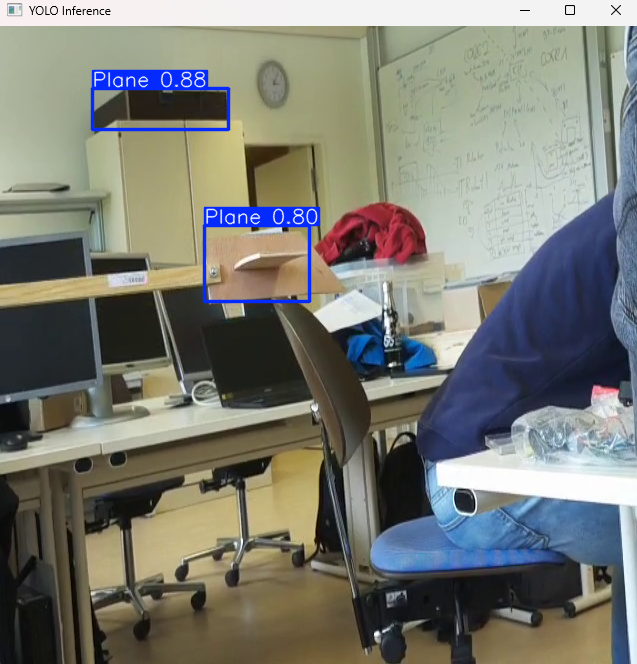
\includegraphics[width=0.9\textwidth,height=6.2cm,keepaspectratio]{images/Python_Inferenz.png}
    \caption{Inferenz in Python mit Ultralytics}
    \label{fig:Screenshot: Inferenz Python mit Ultralytics}
  \end{subfigure}
  \caption{Vergleich Inferenz ONNX C++ und Python}
  \label{tab:Vergleich Inferenz ONNX C++ und Python}
\end{figure}

Wie in \ref{tab:Vergleich Inferenz ONNX C++ und Python} zu sehen ist, sind die Ergebnisse der Inferenz in Python mit der Ultralytics-Bibliothek deutlich besser.
Basierend auf diesen Resultaten wurde entschieden, dass eine weitere Implementierung in C/C++ nicht sinnvoll ist. So fällt besonders die hohe Komplexität, die fehlerhaften Erkennungen, die hohe Einarbeitungszeit hinsichtlich der Projektdauer, aber auch der hohe Aufwand für die Einrichtung einer funktionierenden Laufzeitumgebung ins Gewicht. Mit der Verwendung der Ultralytics Bibliothek fällt ein Großteil dieser Komplexität weg. 

\section{Inferenz des PyTorch-Modells (Jürgens)}

\subsection{Installation der KI-Abhängigkeiten (Jürgens)} 
Neben der reinen Ultralytics-Bibliothek welche mit einer Reihe weiterer Abhängigkeiten installiert wird, ist besonders die Python-Version von \texttt{OpenCV} von Bedeutung. 
OpenCV ist größtenteils in C++ geschrieben, bietet aber auch eine Python-Schnittstelle an. Diese soll dafür verwendet werden, um auf den Kamera-Stream des Raspberry Pi 5 zuzugreifen und bildet die Grundlage für die Inferenz mit dem YOLO-Modell. 
In der Regel kann ein Stream in OpenCV mit der Funktion \texttt{cv2.VideoCapture()} geöffnet werden. Der Stream kann dabei eine angebundene Kamera, eine Videodatei oder auch ein RTSP-Stream sein. Aufgrund fehlender Unterstützung des Kamera-Softwarestacks des Raspberry Pi 5 kann die Kamera nicht direkt mit der Funktion \texttt{cv2.VideoCapture()} geöffnet werden \ref{opencvlibcamera}. Der Test mit einer USB-Kamera dagegen funktionierte problemlos. Da OpenCV eine essenzielle Abhängigkeit in diesem Projekt ist, wurde ein Workaround gefunden in dem die Kamera des Raspberry Pi 5 mittels GStreamer an OpenCV übergeben wird. Eine reguläre OpenCV-Installation mit dem Python Paketmanager PIP enthält standardmäßig keine GStreamer-Unterstützung. Diese muss explizit aktiviert werden, indem OpenCV aus dem Quellcode mit GStreamer-Unterstützung kompiliert wird. Hierbei ist darauf zu achten, dass nicht nur die GStreamer-Bibliothek korrekt installiert und angegeben wird, sondern auch der Python-Interpreter welcher auf dem Raspberry Pi 5 verwendet wird. Die Kompilierzeit kann dabei mehrere Stunden in Anspruch nehmen und ist abhängig von der Leistung des Systems. So hat die Kompilierung und Installation von OpenCV mit GStreamer-Unterstützung etwa 2 Stunden gedauert. 


\subsection{Erstellung \& Evaluierung der GStreamer-Pipeline (Jürgens)}
Die Video-Pipeline wird insgesamt in zwei Kommunikationspartner aufgeteilt. Der erste Kommunikationspartner bildet eine libcamera-vid-Instanz, welche per Kommandozeile gestartet wird. Diese Instanz öffnet die Kamera des Raspberry Pi 5 und sendet diesen Stream an eine angegebene IP-Adresse. \\
Der zweite Kommunikationspartner ist der Empfänger des Kamera-Streams. In diesem Fall stellt das Python-Skript mit der OpenCV Installation inklusive GStreamer-Unterstützung den Empfänger dar. Hier wird das trainierte KI-Modell ausgeführt und auf den Stream angewandt.
Bei der Erstellung der Pipelines wird H264 als Video-Codec und UDP als Transportprotokoll gewählt. Mit dieser Kombination soll eine hohe Performance und eine geringe Latenz erreicht werden.\\
Diese Pipeline überträgt den Kamera-Stream an OpenCV mit einer Latenz von etwa 1 Sekunde. Diese Latenz ist für diese Anwendung inakzeptabel, da die Inferenz des Modells aber auch der Kamerastream so nahe wie möglich an der Echtzeit sein soll. 

\subsection{Inferenz des Modells auf dem Raspberry Pi 5 (Jürgens) \label{sec:inference_raspberry}}
Die Inferenz des Modells erfolgt entsprechend der Dokumentation von Ultralytics. Diese wird in einer Endlosschleife durchgeführt und verarbeitet den Kamera-Stream Bild für Bild. Trotz der relativ guten Hardware des Raspberry Pi 5 (im Vergleich zu älteren Raspberry Pi Systemen) ist die Inferenzzeit und damit Nutzbarkeit dieses Ansatz sehr eingeschränkt. So konnte sehr markantes Ruckeln bei der Anzeige des Kamera-Streams festgestellt werden. Die Ausführung wirkt sich dabei besonders auf die CPU-Last aus. Wie in \ref{fig:CPU und RAM-Auslastung Inferenz RPI5} dargestellt wurde die CPU vom Raspberry Pi 5 teilweise über 90\% ausgelastet. Dieses Verhalten spiegelt sich bei der Performance der KI-Auswertung wieder. So hatte das System trotz der Nutzung des kleinstmöglichen Modells einen sehr geringen Durchsatz (siehe \ref{fig:Zeitanalyse der Inferenz (RPI5)}, grüne Linie). Die Berechnung durch das KI-Modell wurde nach Abstimmung mit Herrn Altmann und dem Team auf einen Laborrechner mit dedizierter Grafikkarte ausgelagert.

\begin{figure}[h]
  \centering
  \begin{subfigure}[b]{\textwidth}
    \centering
    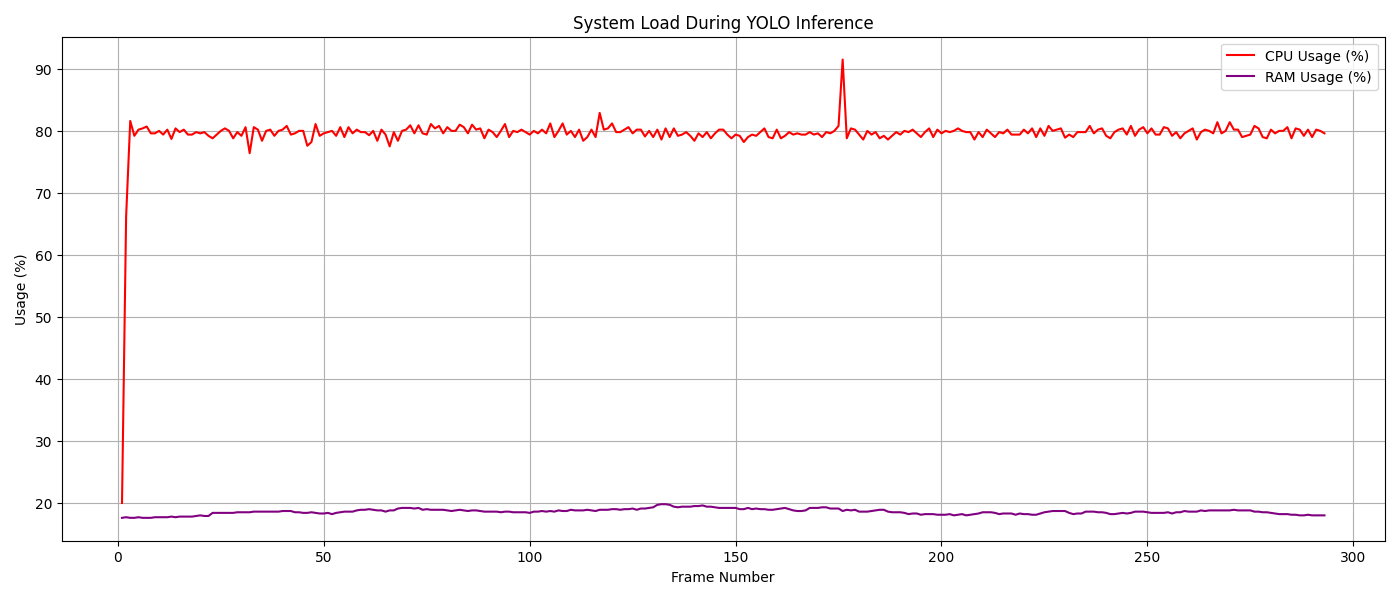
\includegraphics[width=\textwidth,height=5.9cm,keepaspectratio]{images/System_Load_During_Yolo_Inference.png}
    \caption{Systemauslastung während der Inferenz (RPI5)}
    \label{fig:CPU und RAM-Auslastung Inferenz RPI5}
  \end{subfigure}
  \hfill
  \begin{subfigure}[b]{\textwidth}
    \centering
    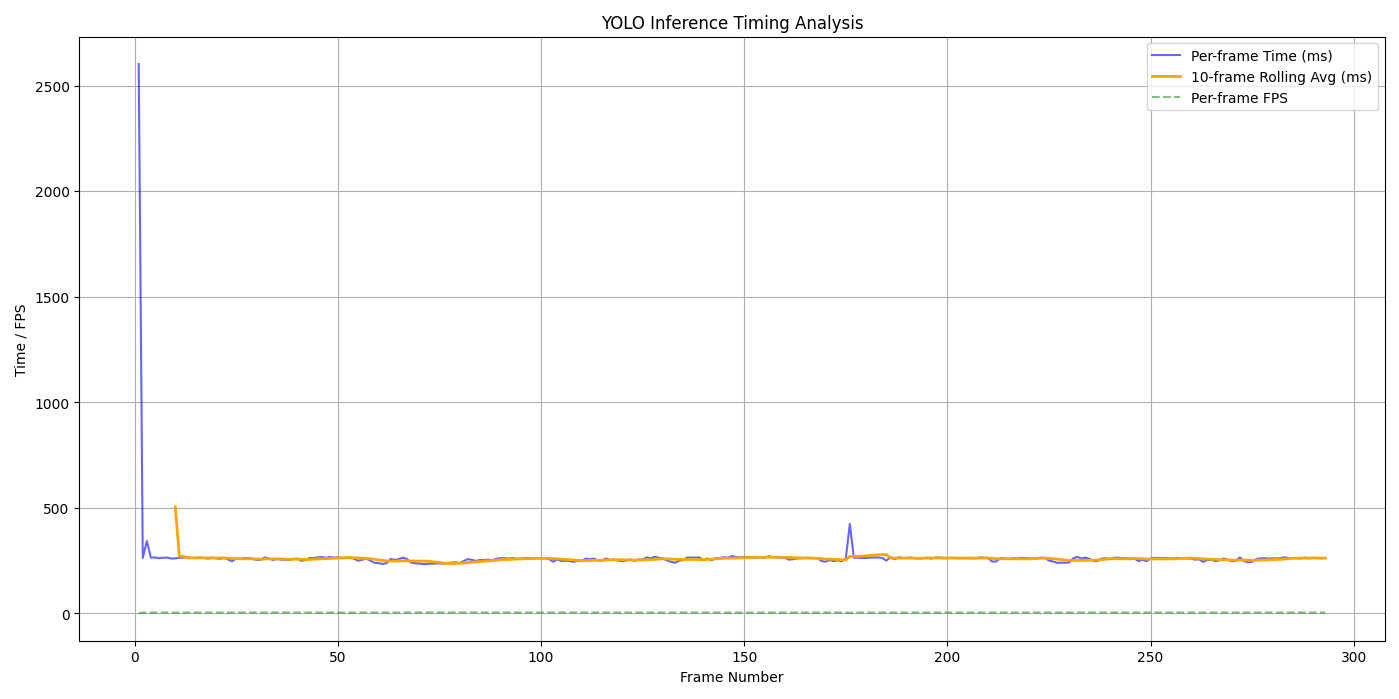
\includegraphics[width=\textwidth,height=6.2cm,keepaspectratio]{images/YOLO_Inference_Timing_Analysis.png}
    \caption{Zeitanalyse der Inferenz (RPI5)}
    \label{fig:Zeitanalyse der Inferenz (RPI5)}
  \end{subfigure}
  \caption{System- und Zeitanalyse während der Inferenz (RPI5)}
  \label{tab:System- und Zeitanalyse waehrend der Inferenz}
\end{figure}


\subsection{Inferenz des Modells auf dem Laborrechner (Jürgens)}
Mit dem Plattformwechsel wurde neben der Ausführungsumgebung ebenfalls das verwendete Modell geändert. So wurde das YOLOv8n Modell durch das YOLOv11 Modell ersetzt, welche hinsichtlich der Performance und Genauigkeit eine kleine Verbesserung bietet.
Die Inferenz des Modells auf dem Laborrechner erfolgt ebenfalls mit der Ultralytics Python-Bibliothek. Anders als auf dem RPI5 läuft die Berechnung des Modells auf der dedizierten Grafikkarte des Laborrechners. Hierbei handelt es sich um eine NVIDIA T1000 Grafikkarte welche die Nutzung von CUDA ermöglicht. Um dieses auch aktiv zu verwenden muss der \texttt{NVIDIA Cuda Compiler Driver} und PyTorch mit CUDA-Unterstützung installiert sein. Die Inferenzzeit des Modells auf dem Laborrechner fällt mit etwa 8 ms deutlich geringer aus und bietet eine flüssigere Anzeige des annotierten Kamera-Streams (siehe \ref{fig:Timing Zusammenfassung CUDA vs RPI5}). 
\begin{figure}[h]
  \centering
  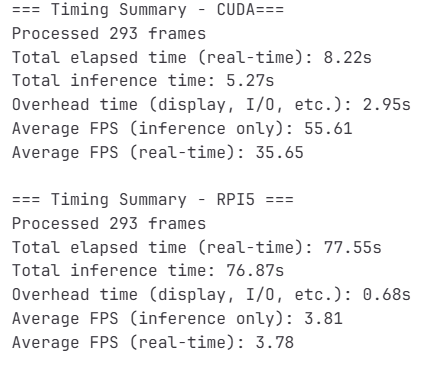
\includegraphics[scale=0.5]{images/Timing_summary.png}
  \caption{Timing Zusammenfassung CUDA vs RPI5}
  \label{fig:Timing Zusammenfassung CUDA vs RPI5}
\end{figure}
\newpage

Durch die Verwendung der dedizierten Grafikkarte wird nun anstelle der CPU die GPU für die Inferenz verwendet. Dies führt zu einer deutlich geringeren Belastung der CPU des Systems (siehe \ref{tab:CPU und RAM-Auslastung CPU vs CUDA})

\begin{figure}[h!]
  \centering
  \begin{subfigure}[b]{\textwidth}
    \centering
    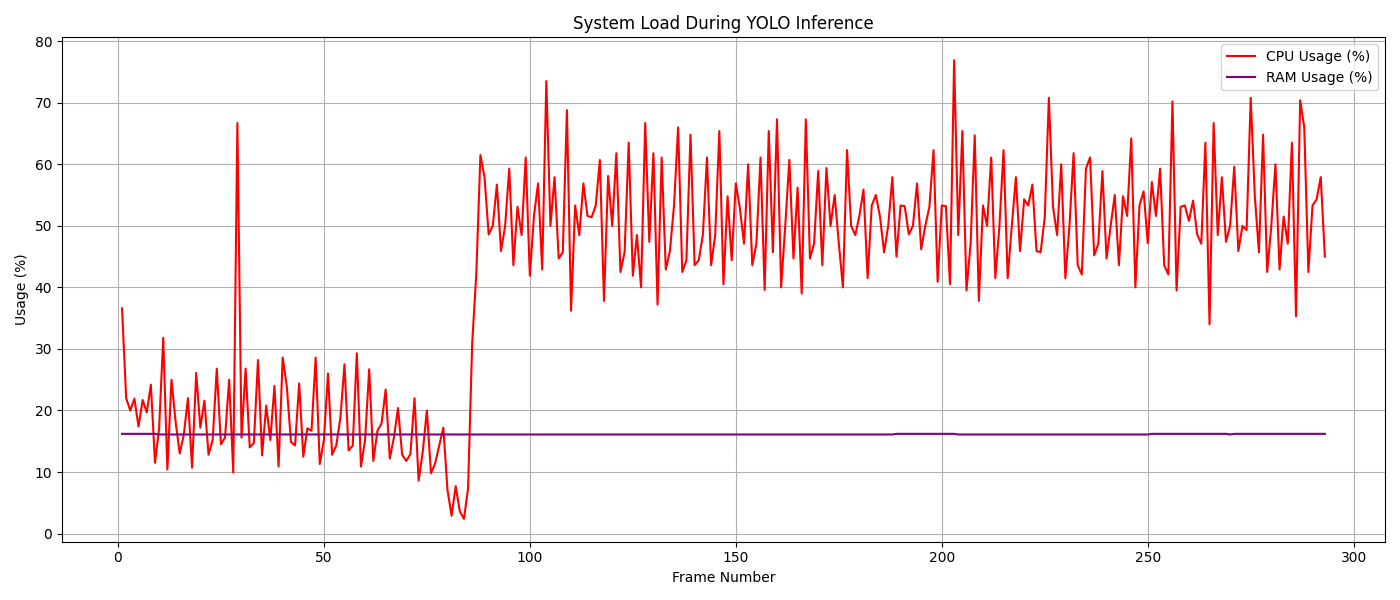
\includegraphics[width=0.9\textwidth,height=5.9cm,keepaspectratio]{images/system_load_plot_CPU_Laborrechner.png}
    \caption{Systemauslastung Laborrechner ohne CUDA}
    \label{fig:CPU und RAM-Auslastung ohne CUDA}
  \end{subfigure}
  \hfill
  \begin{subfigure}[b]{\textwidth}
    \centering
    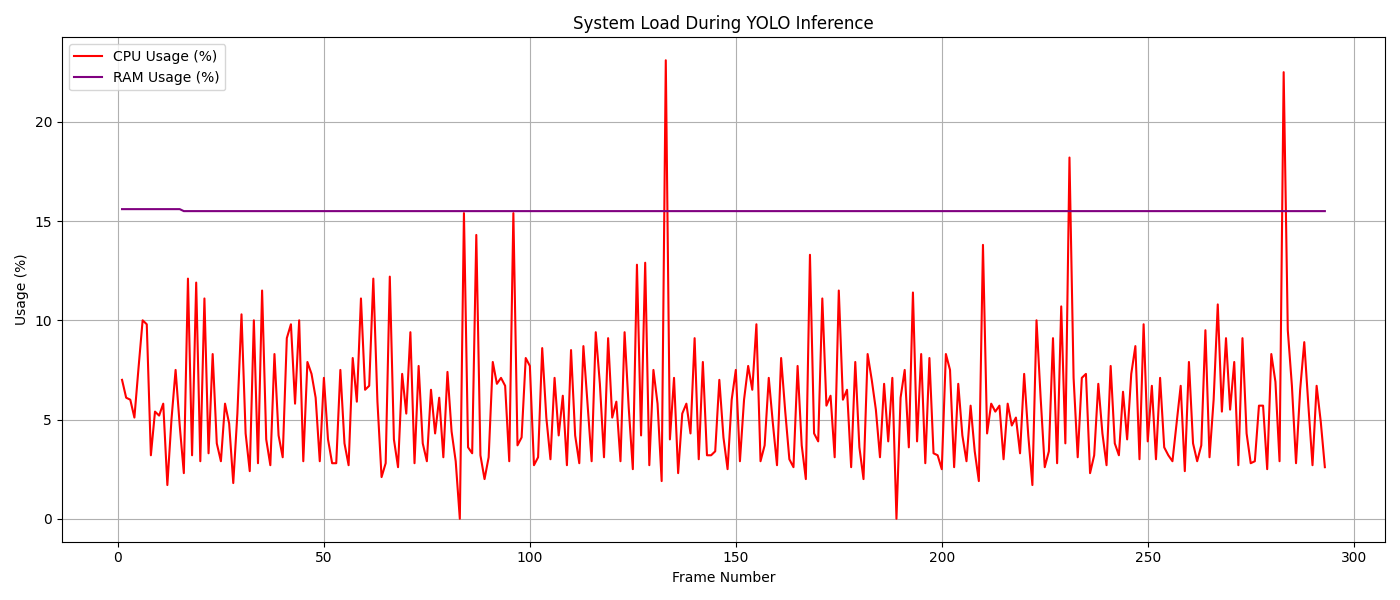
\includegraphics[width=0.9\textwidth,height=6.2cm,keepaspectratio]{images/system_load_plot_CUDA.png}
    \caption{Systemauslastung Laborrechner mit CUDA}
    \label{fig:CPU und RAM-Auslastung mit CUDA}
  \end{subfigure}
  \caption{Vergleich Inferenz ONNX C++ und Python}
  \label{tab:CPU und RAM-Auslastung CPU vs CUDA}
\end{figure}

\newpage

Der Rückgabewert der Inferenz des Modells beinhaltet unter anderem die Koordinaten der Bounding Box, die Klasse und den Konfidenzwert des erkannten Objekts. Die Konfidenz gibt an, zu wie viel Prozent sich das Modell bei dem erkannten Objekt sicher ist. \cite{InferenzResults} 

Diese Informationen können nun direkt für weitere Aktionen verwendet werden. Die detektierte Bounding Box wird dem Frame des Kamera-Streams hinzugefügt und auf dem Bildschirm angezeigt. 